%% 情報学群実験第3,4(C)用のレポートテンプレート
%
\documentclass[a4j,titlepage]{jarticle}
%% プリアンブルここから
\usepackage[dvipdfmx]{graphicx}
\usepackage{url}
\usepackage{comment}
\usepackage{here}
%
\title{\huge 配達支援システム\\
		内部設計書}
\author{第0版\\
        ONO-Systems\\}
\date{\today}

%本文
\begin{document}
\maketitle

%目次
\tableofcontents
\clearpage


\section{開発対象のシステム概要}
本システムは,配達物の配達支援を行うシステムです.主な機能を以下に示します.
\begin{itemize}
\item 利用者への通知機能
\item 配達員の位置情報の表示機能
\item 利用者の選択結果のリアルタイム表示機能
\item 音声読み上げ機能
\end{itemize}


\section{開発環境}
本システムの開発環境を以下に示します.
\begin{itemize}
\item Android アプリケーション\\
  Android Studio ver4.2 とか
\item サーバ\\
  AWS(AmazonWebService)
\item 開発言語\\
  Java, MySQL
\item 文書・コード管理\\
  GitHub
\end{itemize}


\section{動作環境}
\begin{itemize}
\item Android アプリケーション\\
  Android 4.2とか
\item サーバ\\
  AWS(AmazonWebService)
\end{itemize}


\section{コーディング規約}
本プロジェクトのプログラムは、以下の規則を遵守します.
\subsection{コンポーネントやクラスについて}
\begin{itemize}
\item UpperCamelCaseを利用する
\item Component名は最後につける(Activity, Fragment, TextAreaなど)
\item 本プロジェクトで頻繁に利用する名詞は以下の表を用いて命名する(表\ref{termTable}参照)
\begin{table}[htb]
\centering
\caption{本プロジェクトで利用する名詞の英単語表}
\label{termTable}
\begin{tabular}{|ll|}
\hline
外部設計書での名前 & 英単語      \\ \hline
アカウント保持者  & User     \\
利用者       & Customer \\
配達員       & Courier  \\
配達物       & Delivery \\ \hline
\end{tabular}
\end{table}
\end{itemize}

\subsection{変数の命名について}
\begin{itemize}
\item 命名には英語を用いる
\item 名前から役割が読み取れるように命名する
\item グローバル変数に用いる英単語は省略しない(String ⇒ Strなど)
\item LowerCamelCaseを利用する
\item 定数は全て大文字で表し、スネークケースで連結する
\item forやwhileのカウンタ変数には、i,j,kを用いる
\end{itemize}

\subsection{関数の命名について}
\begin{itemize}
\item 意味と英単語の対応付けを統一する(表\ref{namingTable})
\item 名前は動詞で始める
\item LowerCamelCaseを利用する
\begin{table}[htb]
\centering
\caption{命名に使う英単語表}
\label{namingTable}
\begin{tabular}{|lll|}
\hline
意味            & 英単語    & 例                    \\ \hline
真偽値を取得        & is     & \#isCreated          \\
値を代入          & set    & \#setDelivery        \\
引数を含むか判定      & has    & \#hasFragment        \\
特定の動作をしたときに動作 & on     & \#onClick            \\
新しく作る         & create & \#createSubActivity  \\
新しく作る         & new    & \#newDelivery        \\
更新            & update & \#updateDeliveryDate \\
サーバから情報を取得    & fetch  & \#fetchDeliveryList  \\ \hline
\end{tabular}
\end{table}
\end{itemize}

\subsection{コーディングについて}
\begin{itemize}
\item 字下げは半角スペース2つを用いる
\item マジックナンバーは使用しない
\item 安易にネット上のソースコードを利用しない
\item classやif、whileなどのブロック始点のブラケット('\{')は改行せずに、半角スペースを空けて記述する
\item 機能が完成したとき(Pull Requestsを出すとき)にデバッグ用のコードを残さない
\end{itemize}

\subsection{コメントについて}
\begin{itemize}
    \item 複雑な処理はコメントをつける
    \item メソッドにはコメントをつける
    \item TODO:など、コードの説明でないコメントはPullRequestsを出すときには消す
\end{itemize}

\section{ネットワーク設計}
本システムのネットワークは図\ref{fig:n_d}のように構成されます.

\begin{figure}[H]
 \begin{center}
  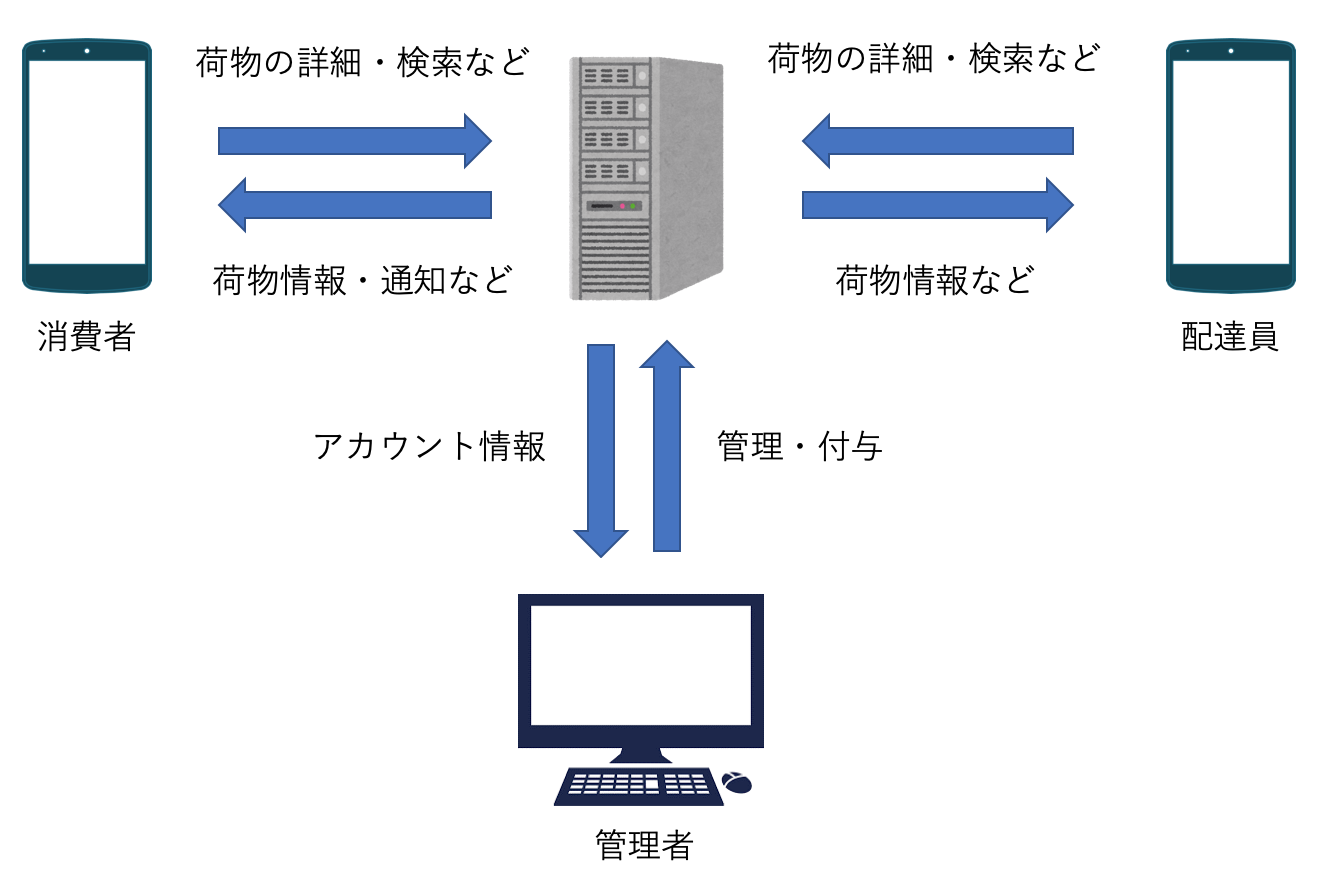
\includegraphics[width=140mm]{Network_Diagram.png}
  \caption{ネットワーク構成図}
  \label{fig:n_d}
 \end{center}

\end{figure}

\section{Android モジュール設計}
\subsection{モジュール構成}

\subsection{モジュール仕様}


\section{Server モジュール設計}
\subsection{モジュール構成}
\subsection{モジュール仕様}



\section{データベース設計}
本システムではデータベースにAWS(AmazonWebService)を使用します.\\
ER図など
\subsection{各テーブルの詳細}
本システムのデータベースには,5個のデータテーブルを用います.各データテーブルの役割と属性を以下に示します.
\subsubsection{消費者テーブル}
消費者テーブルでは,消費者に関する情報を管理します.このテーブルのデータテーブルを表\ref{customer}に示します.
\begin{table}[htb]
  \caption{消費者テーブル}
  \label{customer}
  \begin{center}
    \begin{tabular}{|c|c|c|c|c|c|} \hline
      属性 & データ型/長 & NULL & Key & 初期値 & その他 \\ \hline \hline
      customer\verb|_|id & int(9) unsigned & NO & PRIMARY & NULL & auto\verb|_|increment\\ \hline
      name & varchar(64) & NO &   &  & \\ \hline
      mail & varchar(64) & NO &   &  & \\ \hline
      tel & varchar(11) & YES &   & NULL & \\ \hline
      address & varchar(128) & YES &   & NULL & \\ \hline
      hash & varchar(255) & NO &   &  & \\ \hline
      salt & varchar(255) & NO &   &  & \\ \hline
    \end{tabular}
  \end{center}
\end{table}

\subsubsection{配達者テーブル}
配達者テーブルでは,配達者に関する情報を管理します.このテーブルのデータテーブルを表\ref{driver}に示します.
\begin{table}[htb]
  \caption{配達者テーブル}
  \label{driver}
  \begin{center}
    \begin{tabular}{|c|c|c|c|c|c|} \hline
      属性 & データ型/長 & NULL & Key & 初期値 & その他 \\ \hline \hline
      driver\verb|_|id & int(9) unsigned & NO & PRIMARY & NULL & auto\verb|_|increment\\ \hline
      name & varchar(64) & NO &   &  & \\ \hline
      mail & varchar(64) & NO &  &  & \\ \hline
      tel & varchar(11) & YES &  & NULL & \\ \hline
      store\verb|_|code & varchar(64) & YES &   & NULL & \\ \hline
      account\verb|_|type & int(1) unsigned & YES &   & NULL & \\ \hline
      hash & varchar(255) & NO &   &  & \\ \hline
      salt & varchar(255) & NO &   &  & \\ \hline
    \end{tabular}
  \end{center}
\end{table}

\subsubsection{商品テーブル}
商品テーブルでは,商品に関する情報を管理します.このテーブルのデータテーブルを表\ref{delivery}に示します.
\begin{table}[htb]
  \caption{商品テーブル}
  \label{delivery}
  \begin{center}
    \begin{tabular}{|c|c|c|c|c|c|} \hline
      属性 & データ型/長 & NULL & Key & 初期値 & その他 \\ \hline \hline
      slip\verb|_|number & varchar(12) & NO & PRIMARY & NULL & \\ \hline
      name & varchar(64) & NO &   &  & \\ \hline
      address & varchar(128) & NO &   &  & \\ \hline
      ship\verb|_|from & varchar(64) & YES &  & NULL & \\ \hline
      time & varchar(10) & YES &   & NULL & \\ \hline
      delivered\verb|_|status & int(1) unsigned & NO &   & 0 & \\ \hline
      receivable\verb|_|status & int(1) unsigned & NO &  & 0 & \\ \hline
      customer\verb|_|id & int(9) unsigned & NO & MULTIPLE & NULL & \\ \hline
      driver\verb|_|id & int(9) unsigned & NO & MULTIPLE & NULL & \\ \hline
    \end{tabular}
  \end{center}
\end{table}

\subsubsection{管理者テーブル}
管理者テーブルでは,管理者に関する情報を管理します.このテーブルのデータテーブルを表\ref{manager}に示します.
\begin{table}[htb]
  \caption{管理者テーブル}
  \label{manager}
  \begin{center}
    \begin{tabular}{|c|c|c|c|c|c|} \hline
      属性 & データ型/長 & NULL & Key & 初期値 & その他 \\ \hline \hline
      manager\verb|_|id & int(1) unsigned & NO & PRIMARY & NULL & auto\verb|_|increment\\ \hline
      name & varchar(64) & NO &   &  & \\ \hline
      mail & varchar(64) & NO &  &  & \\ \hline
      store\verb|_|code & varchar(64) & YES &   & NULL & \\ \hline
      account\verb|_|type & int(1) unsigned & YES &   & NULL & \\ \hline
      hash & varchar(255) & NO &   &  & \\ \hline
      salt & varchar(255) & NO &   &  & \\ \hline
    \end{tabular}
  \end{center}
\end{table}

\subsubsection{地図テーブル}
地図テーブルでは,地図に関する情報を管理します.このテーブルのデータテーブルを表\ref{map}に示します.
\begin{table}[htb]
  \caption{地図テーブル}
  \label{map}
  \begin{center}
    \begin{tabular}{|c|c|c|c|c|c|} \hline
      属性 & データ型/長 & NULL & Key & 初期値 & その他 \\ \hline \hline
      slip\verb|_|number & varchar(12) & NO & MULTIPLE & NULL & auto\verb|_|increment\\ \hline
      lat & double(8,6) & YES &   & NULL & \\ \hline
      lng & double(9,6) & YES &   & NULL & \\ \hline
    \end{tabular}
  \end{center}
\end{table}


\section{バージョン管理規約}
本システムの開発では,Github を用いてファイルの管理を行います.Github を使用する際には,以下の規則を遵守します.
\begin{itemize}
\item ドキュメント関連の資料は,onosystem-doc で管理する
\item Android のソースコードは,onosystem-android で管理する
\item Server のソースコードは,onosystem-server で管理する
\item 編集作業を行う際には,ブランチを切ってコミットする
\item 開発用ブランチの名前は,「dev\verb|_|○○(開発している機能名)」にする
\item 細かい頻度でコミットする(1日の作業ごとに纏めてコミットしない)
\item コミットのコメントはわかりやすい内容にする
\item Pull Requests されたものを確認し,評価をリアクションのアイコンを追加することで示す
\item Pull Requests に対して高評価が3つ以上ある場合には master に Merge する
\end{itemize}

\end{document}
